
\documentclass{beamer}
\usepackage{graphicx}
\graphicspath{{images/}}


\author{Sam Barrett, 1803086}
\title{{Master's Project Presentation} \\ \texorpdfstring
        {
\includegraphics[scale=0.1]{uobcrest.jpg}}
    }
\institute{{University of Birmingham}}
\date{\today}

\begin{document}

\begin{frame}
\titlepage
\end{frame}


\section{My Topic}
\begin{frame}
    \frametitle{My Topic}
    \framesubtitle{Applications of Genetic Algorithms on Fully Autonomous Road Networks}

    \begin{itemize}

        \item Semi-autonomous vehicles are becoming more prevalent 
        \item Roads are becoming more congested
        \item Fully autonomous vehicle trials have been legal in parts of the US since 2015\cite{AutonomousVehiclesSelfDriving}, with the UK set to follow by next year (2021)\cite{UKWantsFully2019}
        \item Much of the current research into autonomous vehicle routing focuses on environments where human drivers are still present
        \item By removing the human element and working on theoretical \textit{fully autonomous road networks} we can make many useful assumptions about the behaviour of other vehicles

    \end{itemize}
\end{frame}


\section{Literature}
\begin{frame}
    \frametitle{Literature Review}
\end{frame}


\section{Methods}
\begin{frame}
    \frametitle{Methods}
    \framesubtitle{Language Choice} 
    Not final but preliminary implementations have used Julia\cite{JuliaProgrammingLanguage}
    \begin{itemize}
        \item C-like performance
        \item Python \& Matlab -like syntax
        \item Matlab like matrices 
        \item Allows for both OO and functional approaches to problems
        \item Allows for use of Unicode in variable \& function names so implementations of advanced mathematical expressions are much more readable
    \end{itemize}
\end{frame}

\begin{frame}
    \begin{figure}[Example Julia code]
        \centering
        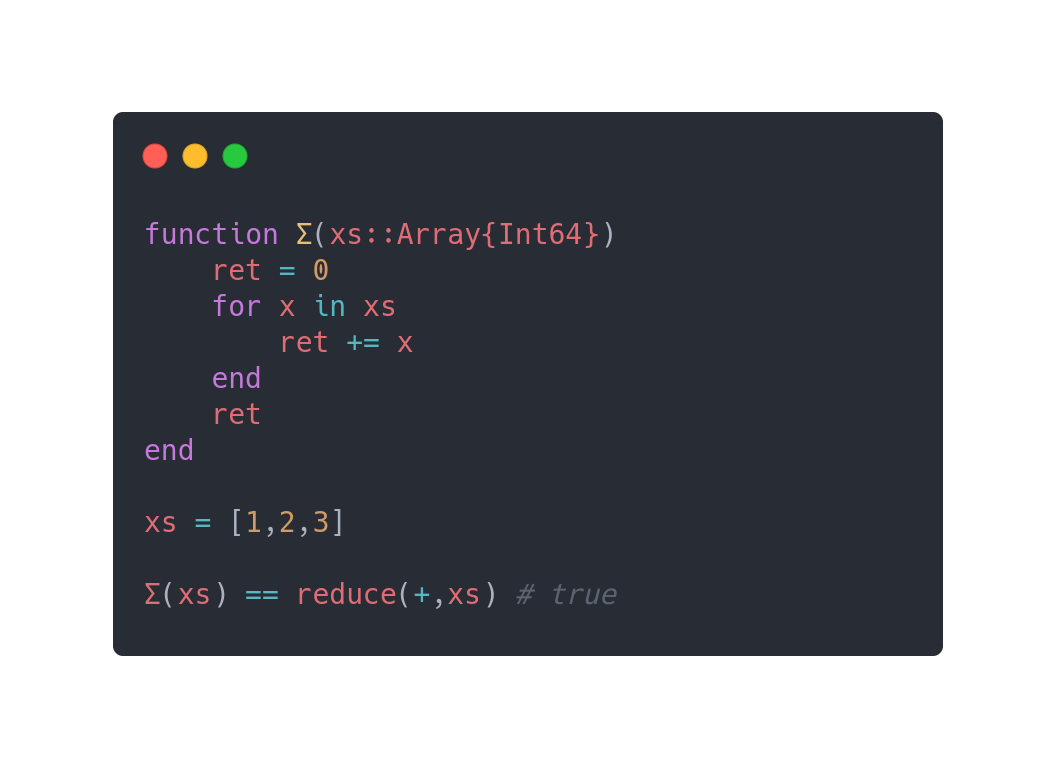
\includegraphics[scale=0.26]{juliaeg.png}
        \caption{Example Julia code}%
        \label{fig:name}
    \end{figure}
\end{frame}

\begin{frame}
Alternatives include Rust and Python3

Python3:
\begin{itemize}
    \item Simple syntax
    \item Wealth of stress-tested libraries
        \item Slow relative to alternatives
            \item unable to compile to binary format
                \item Has some functional capabilities
                    \item Has some static typing ability
\end{itemize}
Rust:
\begin{itemize}
    \item Slower to prototype in as stricter type system to guarantee memory safety
        \item Very performant
\end{itemize}
\end{frame}

\section{Bibliography}
\begin{frame}
\frametitle{References}
\bibliographystyle{abbrv}
\bibliography{lib}
\end{frame}

\end{document}
